\section{Vorlesung 18.11.2016}
\subsection{Graphen in der Ebene und planare Graphen}
\textbf{Topologie}
\begin{itemize}
	\item euklidische Ebene: $\mathbb{R}^2$ 
	\item Liniensegmente \{ p+x(q-p)\} mit p,q $\in \mathbb{R}^2$ und $p \neq q$
	\item homöomorphisch (bijektive stetige Abbildung) zum Einheitskreis
	\item Polygonzug (zusammenhängende Folge von Kanten)
\end{itemize}
\textbf{\textit{Theorem}: Jordan'scher Kurvensatz}\newline
Für jedes Polygon $P \subseteq \mathbb{R}^2$ hat $\mathbb{R}^2\notin P$ zwei Regionen, wobei P die Grenze bildet\newline $\rightarrow$ definiertes außen und innen \newline
\textbf{Lemma}\newline
Seien $P_1, P_2, P_3$ Polygonzüge mit den Endpunkten x und y, so hat $\mathbb{R}^2 \notin \{ P_1 \cup P_2 \cup P_3\}$ drei Facetten mit den Grenzen $P_1, P_2, P_3$ (ohne die Endpunkte x und y): 
\begin{itemize}
	\item{} $b_1 := P_1 \cup P_2$
	\item{} $b_2 := P_1 \cup P_3$
	\item{} $b_3 := P_2 \cup P_3$ 
\end{itemize}
$\rightarrow$ falls $P_4$ ein Polygonzug zwischen $\dot{P_1}$ und $\dot{P_3}$ mit $\dot{P_4}, \dot{P_2} \subset \mathbb{R}^2 \notin \{ P_1 \cup P_3\}$ ist, so schneiden sich $P_4$ und $P_2 (\dot{P_4} \cap \dot{P_2}) \neq 0$ \newline

\textbf{\textit{Graph in Ebene:}} \newline
Ein Graph in der Ebene (V,E) hat folgende Eigenschaften
\begin{itemize}
	\item[1] $V \subset \mathbb{R}$
	\item[2] Jede Kante sei ein Polygonzug zwischen zwei Knoten
	\item[3] unterschiedliche Kanten haben unterschiedliche Mengen von Knoten
	\item[4] das innere einer Kante enthält keinen Knoten und keinen Punkt einer anderen Kante 
\end{itemize}
somit ist ein Graph in der Ebene \textit{kreuzungsfrei} (auch siehe oben $\Rightarrow$ Kreuzungszug)
\\\\
\textbf{\textit{Facette}}\newline
Falls G ein Graph in der Ebene ist, so sind die Regionen $\mathbb{R}^2 \notin G$ die Facetten. Die äußere Facette liegt außerhalb des Graphen und die anderen Facetten liegen per Definition innerhalb. \newline

\newpage
\textbf{Lemma} \newline
Sei G ein Graph in der Ebene, $f \in F(G)$ eine Facette und $H \subseteq G$ ein Subgraph, so gilt:
\begin{itemize}
	\item H hat eine Facette f' mit f $\subseteq$ f'
	\item Falls der Rand von f $\subset$ H ist, dann ist f' = f
\end{itemize}

\textbf{\textit{Theorem:} Eulersche Formel} \newline
Sei G ein verbundener Graph in der Ebene mit n Knoten, m Kanten und l Facetten, so gilt: \textbf{n - m + l = 2} \newline

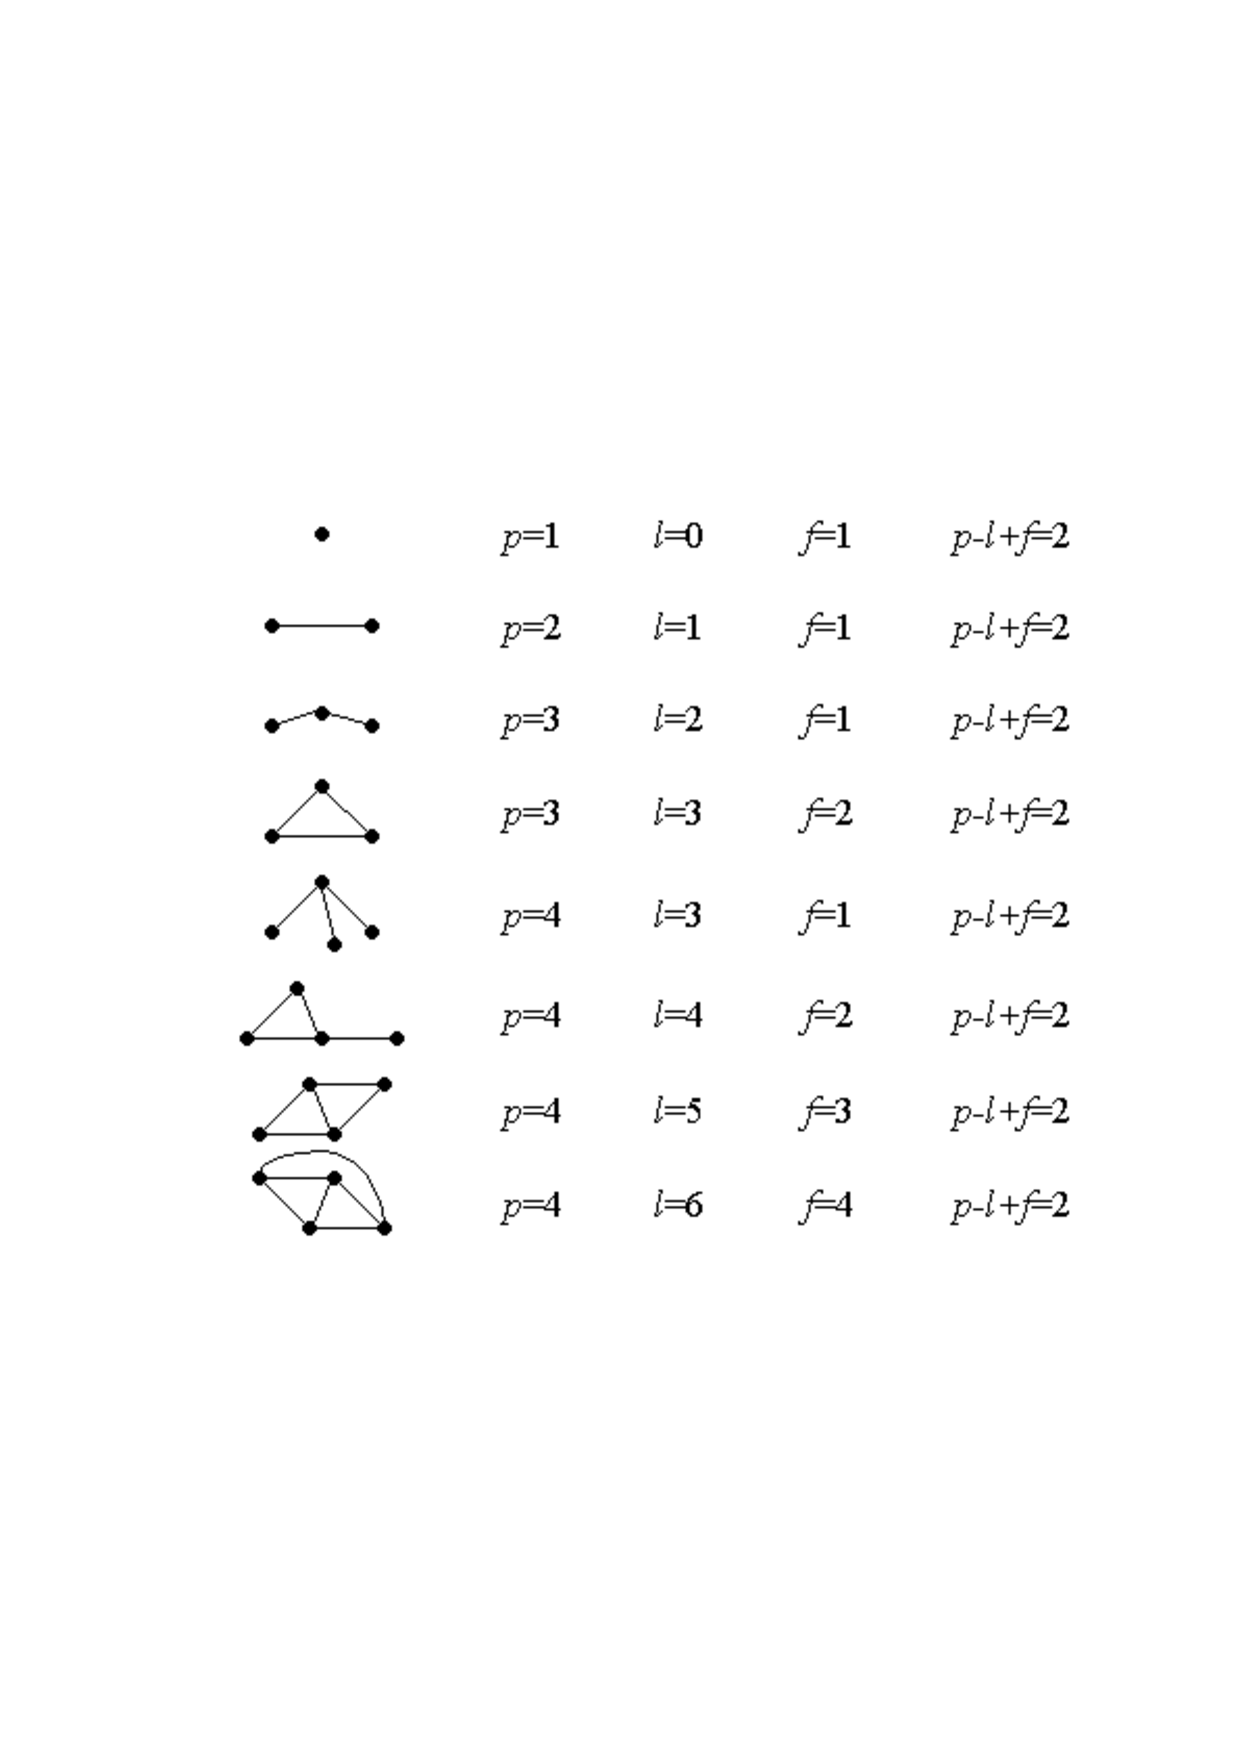
\includegraphics[scale=0.5]{lectures/161118/pix/planareGraphenElementar.pdf}\newline

\textbf{Beweis} \newline
Sei n fixiert $\rightarrow$ induziere über m.
\begin{itemize}
	\item if $m < n -1:$ Graph ist nicht verbunden
	\item if $m = n -1:$ Graph ist ein Baum
	\item if $m \ge n:$ Sei $e \in E(G)$ Kante auf einem Kreis, dann ist G' = G-e \textcolor{red}{-$|\setminus$}\\ $\rightarrow$ e liegt auf der Grenze zweier Facetten $f_1 und f_2$ von G und es gibt eine Facette $f_e$ von G', die $\dot{e}$ enthält. 
\end{itemize}
Zeige, dass $F(G) \notin \{f_1, f_2\} = F(G') \notin \{f_e\}$, womit G' eine Facette und eine Kante weniger hat als G. \textcolor{red}{-$|\setminus$}\newline
$\rightarrow$ Das entfernen einer Kante kombiniert 2 Facetten \newline
$\rightarrow$ Fügt man einen Knoten hinzu so wird auch eine Kante hinzugefügt \newline
$\rightarrow$ $|V'|=|V|+1$ und $|E'|=|E|+1$ $\rightarrow$ q.w.e.d. \newline

\newpage
\textbf{Korollar 1}
\begin{itemize}
	\item[1)] Ein kreuzungsfreier verbundener Graph in der Ebene mit $n \ge 3$ Knoten hat maximal 3n - 6 Kanten
	\item[2)] Jede Triangulation mit n Knoten hat genau 3n - 6 Kanten 
\end{itemize}
\textbf{Korollar 2(nach Kuratowski)} \newline
Ein Graph in der Ebene hat weder $K_5$ noch $K_{3.3}$ als topologischen Minor ($K_5$ und $K_{3.3}$ sind nicht mehr kreuzungsfrei zeichenbar).\newline
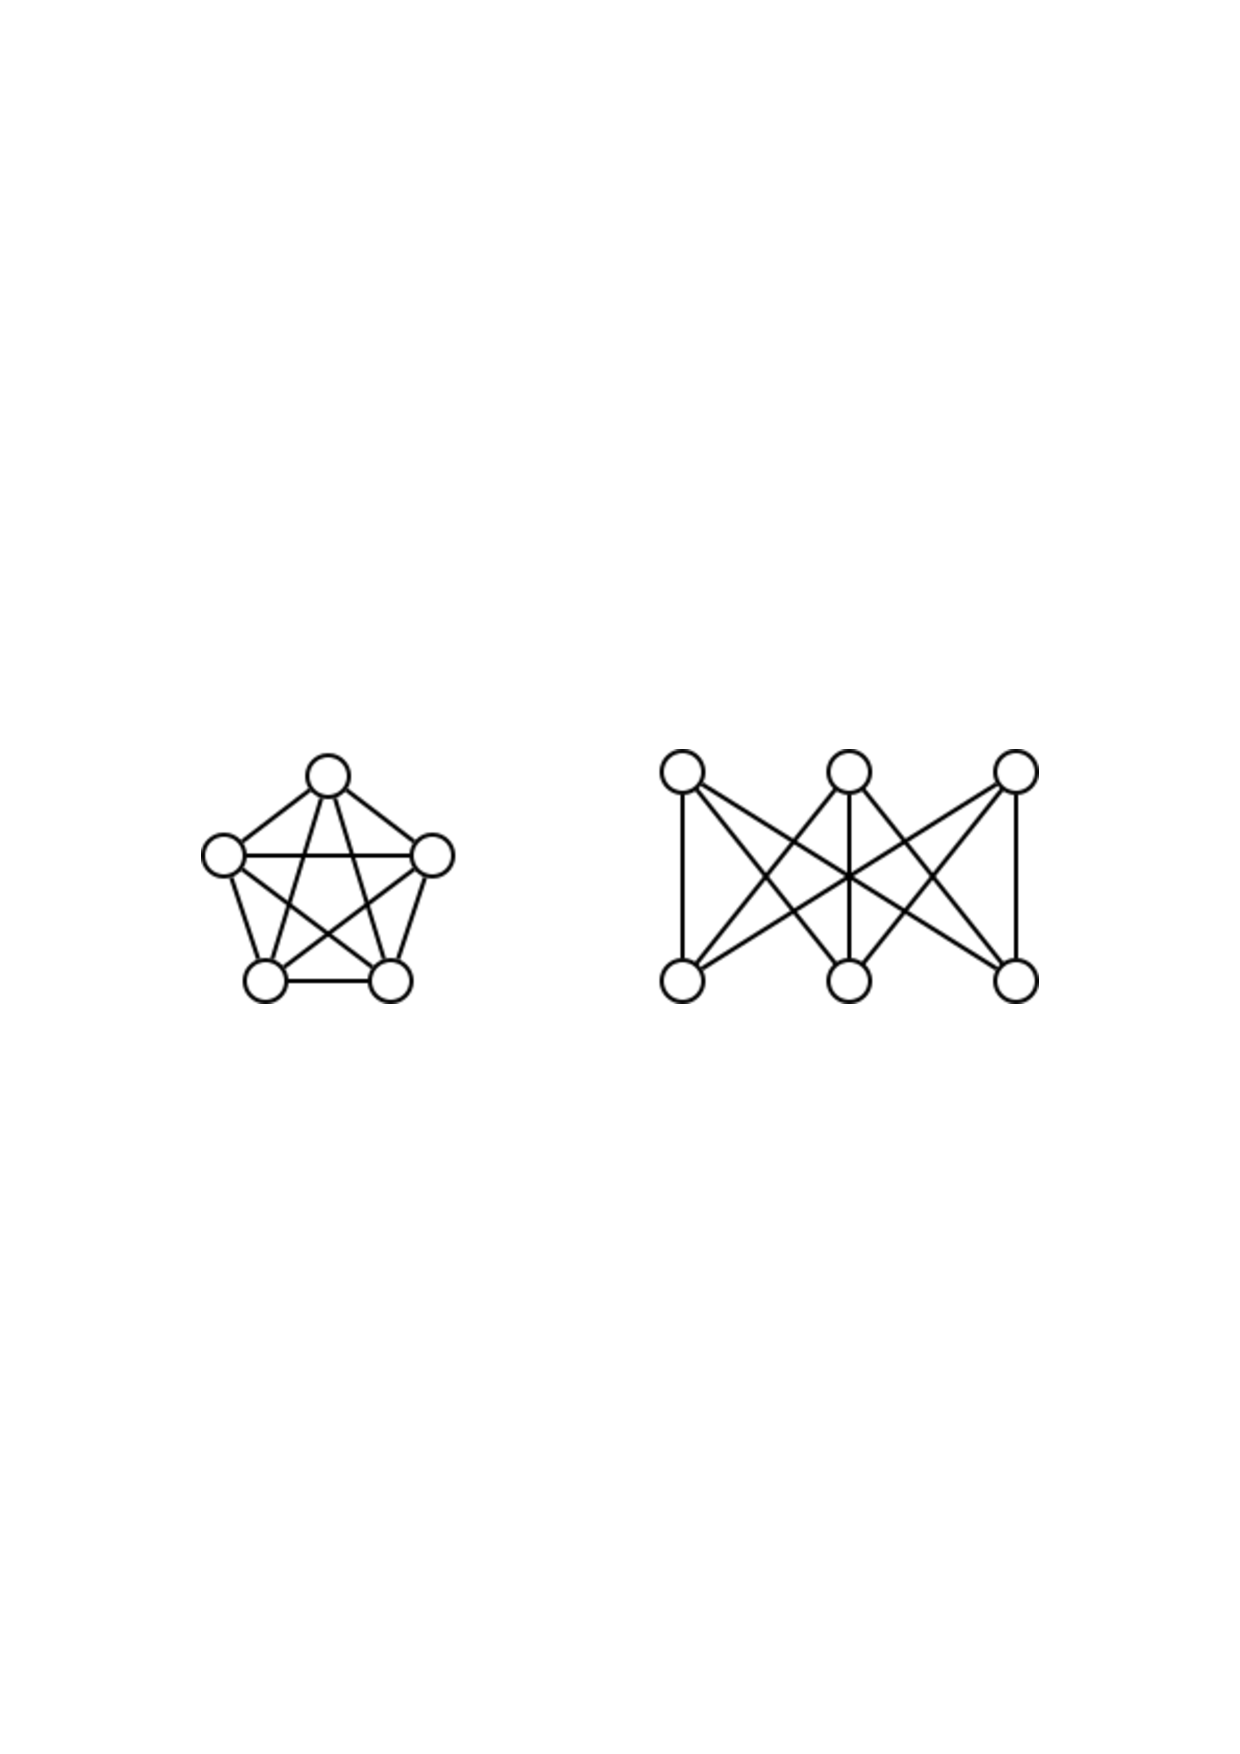
\includegraphics[scale = 0.5]{lectures/161118/pix/K33+K5.pdf} \newline
\textbf{\textit{Minor}}\newline
H ist ein Minor von G, falls G in H durch folgende Operationen transformiert werden kann:
\begin{itemize}
	\item G - e, e $\in$ E(G)
	\item G-v, v $\in$ V(G) (hierbei werden auch nichtverbundene Kanten gelöscht)
	\item Kontraktion von e $\in$ E(G) mit e = {u,v}, u,v $\in$ V(G), wobei u,v zu einem Knoten vereinigt werden und dieser zu allen Nachbarn inzident wird.
\end{itemize}
\textbf{\textit{planarer Graph}} \newline
Ein Graph G sei planar, wenn er folgende Eigenschaften erfüllt: 
\begin{itemize}
	\item Eine endliche Anzahl von Facetten bildet eine Kreisbasis
	\item jede Kante, die zwei Kreisen zugehörig ist, heißt innere Kante
	\item jede Kante, die einem Kreis zugehörig ist, heißt äußere Kante
\end{itemize}
\textbf{\textit{2-Basis}}\newline
Jede Kante ist genau 2 mal in den Kreisbasen vertreten.\newline
 
\textit{Konstruktion 2-Basis}
\begin{itemize}
	\item F = $\bigoplus\limits_{c \in B} c$ Rand der äußeren Facette (äußerer Rand) mit B=Menge von Kreisen
	\item 2-Basis = $B \cup F$ 
\end{itemize}

\newpage
\textbf{\textit{Satz von Mc Lane}}\newline
G ist planar, wenn G auch eine 2-Basis hat.

\textbf{Beweis:}
\begin{itemize}
	\item[1] B sei 2-Basis von G und G sei nicht planar 
	\item[] nach Kuratowski ist Subdivision von $K_5$ oder $K_{3,3}$ $H \subset G$ möglich \newline Behauptung: $\rightarrow$ H hat ebenfalls eine 2-Basis \newline
	
	\item[2] $G \notin e, \forall e$ hat eine 2-Basis
	\item[] es ist nur in einem Kreis $C \in B$ vorhanden, womit $B \notin C$ entsteht.
	\item[] e ist in zwei Kreisen vorkommend, womit $B \notin \{C_1, C_2\} \cup \{ C_1 \oplus C_2\}$ eine 2-Basis ist \newline $\rightarrow$ somit haben alle Teilgraphen eine 2-Basis. Da die Behauptung belegt ist $\Rightarrow$ \textbf{Widerspruch}
\end{itemize}
\textit{\underline{zyklometrische Zahl:}} Die Anzahl der Bassiselemente einer Kreisbasis\\
$\mu(G)=|E(G)| - |V(G)| + k(G)$\\
mit k(G) = \#Zusammenhangskomponenten
\\
\newline
\textbf{\textit{Beispiel:} vollständiger Graph $K_5$}
\begin{itemize}
	\item $|V| = 5 ; |E| = 10$
	\item 2-Basis mit 5 inneren und 5 äußeren Kanten
	\item $\mu(K_5)$ = -5 + 10 +1 = 7
	\item 2-Basis hat demnach (2n -6)*7 Kanten = 21 Kanten $\rightarrow$ \newline \textbf{falsche Aussage}
\end{itemize}	
\textbf{\textit{Beispiel:} bipartiter Graph $K_{3,3}$}
\begin{itemize}
	\item $|V| = 6 ; |E| = 9$
	\item $\mu(K_{3,3})$ = -6 + 9 +1 = 4
	\item 2-Basis hat demnach (2n -6)*4 Kanten = 20 Kanten $\rightarrow$ \newline \textbf{falsche Aussage}
\end{itemize}
\textbf{Planaritätstest}
\begin{itemize}
	\item[1] zähle die Kanten 
	\item[2] Tiefensuche $\rightarrow$ Konstruiere einen Spannbaum
	\item[3] Teste für Kanten e $\leftarrow G \notin T$, ob $K_5$ oder $K_{3,3}$ entsteht.
\end{itemize}